\chapter{Introduction}

\section{LTE systems}

LTE stands for Long-Term Evolution and it is a standard wireless data communication technology for mobile devices and data terminals.
The main aim of LTE is to facilitate low response time and high throughput supporting flexible bandwidth deployments.

The main components of LTE architecture are as follows:

\textbf{UE:} 
User Equipment represent the terminal devices which deal with modules like data communication and terminating data channels.

\textbf{E-UTRAN:} 
Evolved UMTS Terrestrial Radio Access Network are evolved base stations(eNB) which send and receive radio transmissions from the user equipment using the digital and analogue signal processing.

\textbf{EPC:}
Evolved Packet Core  deals with network management and gateway servicing modules.
\begin{figure}[ht!]
        \centering
        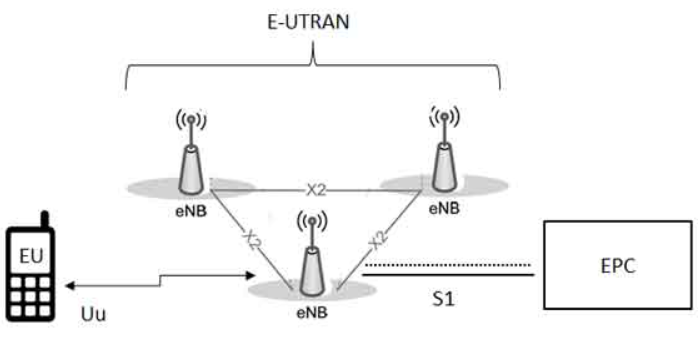
\includegraphics[scale=0.60]{lte_diagram.PNG}
        \\\caption{High-level architecture of LTE systems}
        \label{lte}
\end{figure}


\section{Queuing systems}

Queuing systems deal with the mathematical study of congestion. Generally, the study of servicing requests from customers/entities arriving in a queue fashion at a facility is called queuing theory.
Examples: Ticket booking, customer service centers.

\section{Importance of queuing theory in LTE systems}

With growing modern internet applications and mobile devices, there is a spike in the usage of cellular networks. So it has become very important to investigate and analyze the performance of LTE networks.

Here eNB acts as a server and requests from wireless devices arrive at eNB.
So we can treat the LTE network as a queuing system. The terminal wireless devices use protocols like up-link and down-link for data transfer in LTE networks.

Some important metrics of LTE networks such as waiting delay and block probability are analyzed using queuing theory.

Thus it is very important to study Queuing systems to understand LTE systems and how applications with different burst patterns effect LTE network performance.

\begin{definition}\label{memoryless property}
A process is memory-less if the system forgets the state constantly i.e. probabilities are not influenced by the history of the process. A random variable G is memory-less if the distribution satisfies the property:
\[
P(G>a+b | G>a) = P(G>b)
\]
This property is also referred to as Markov property.
\end{definition}
\begin{definition}\label{poisson process}
A stochastic counting process S(t) with rate $\lambda>0$ is a Poisson process if it satisfies with the following properties:
 \\a. $S(0) = 0.$
 \\b. $S(t)$ has independent increments
 \\c. The count of arrivals in any time span of length $t>0$ follows the distribution Poisson($\lambda t$).
\end{definition}

\begin{definition}
\textbf{Birth death Process:}
When a service request arrives at a queue system, it is allocated a resource and eventually, the customer leaves the system after the service. This is called a birth-death process. Each request arrival is considered as birth and each served customer is considered as death.
\end{definition}

\begin{figure}[ht!]
        \centering
        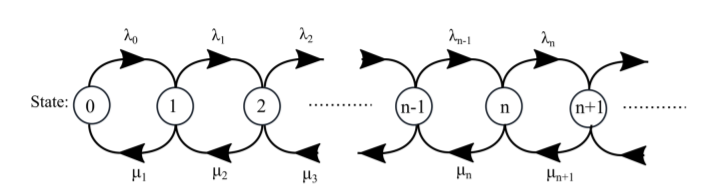
\includegraphics[scale=0.60]{birth_death.png}
        \\\caption{Figure showing the transitions in birth-death process}
        \label{birth-death}
\end{figure}

The arrival rate of customers($\lambda$) and service rate($\mu$) are constant or state-dependent.
Mathematical models of queuing systems are studied using the birth-death framework.

\begin{definition}
\textbf{Little’s Law:}
The fundamental relationship between the three parameters $\lambda$(arrival rate), L(length of the system), W(waiting time in the system)
\[
L = \lambda W
\]
\end{definition}

\section{Queuing models}
Queuing systems are mainly characterized by the arrival of requests, the service mechanism, and queuing discipline

\begin{definition}\label{kendall notation}
Kendall notation is a standard system used in queuing systems to describe a queuing model with three factors A/S/c. Sometimes also referred to as A/S/c/K/N/D.
\\A: Arrival process.
\\S: Servicing process.
\\c: Number of service channels.
\\K: Length of the queue.
\\N: Customer population
\\D: Service discipline
\end{definition}

\subsection{Simple Markovian queues}
\textbf{Single server Queues:}
\\\textbf{M/M/1 model:}
M/M/1 is a simple markovian birth-death process consisting a single server. Arrival and service rates are state independent. Inter-arrival time and service times for M/M/1 queues follow exponential distributions.
\[
d_{arr}(t) = \lambda e^{-\lambda t}
\]
\[
d_{ser}(t) = \mu e^{-\mu t}
\]
$\lambda$: The rate of arrival.
\\$\mu$: The rate of service.
\begin{figure}[ht!]
        \centering
        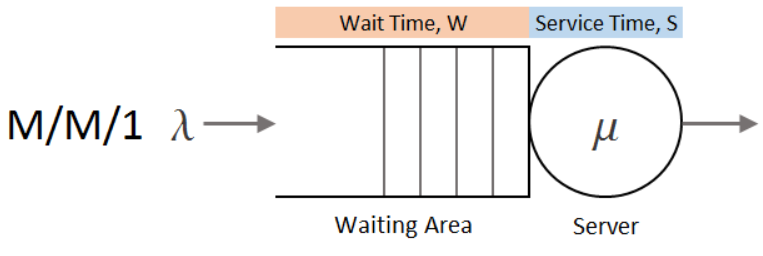
\includegraphics[scale=0.60]{mm1diagram.PNG}
        \\\caption{M/M/1 queue}
        \label{mm1}
\end{figure}

\begin{theorem}
An exponential random variable S has the memory-less property.
\end{theorem}

\begin{proof}
From Bayes theorem, 
\[
P(S > a+b| S > b) =\frac{P(S > a+b, S > b)}{P(S > b)}
=\frac{P(S > a+b)}{P(S > b)}
=\frac{e^{-\lambda(a+b)}}{e^{-\lambda b}}
= e^{-\lambda a}.
\]
\[
 P(S > a+b | S > b) = P(S>a)
\]
Implies exponential random variable is memoryless
\end{proof}

Let $P_n$ be the probability for the system in long-term to stay in state n as shown in Figure \ref{birth-death}.

For a small period of time h,
The steady state probability of the system to stay in state n at time t+h (infinitesimally small h) from the birth-death state figure \ref{birth-death} gives 3 cases:
\begin{itemize}
  \item From state n-1 with one request and no service
  \item From state n+1 with no request and one service
  \item From state n with no request and no service
\end{itemize}

Mathematically written,
\[
P_n(t+h) = P_{n-1} (t)\lambda h(1-\mu h) + P_{n+1} (t)(1-\lambda h)\mu h + P_n(t)(1-\lambda h)(1-\mu h)
\]
For steady state,
\[
\frac{P_n(t+h)-P_n(t)}{h} = 0
\]
\[
 P_{n-1}(t)\lambda + P_{n+1}(t)\mu - P_{n-1}(t)(\lambda+\mu)=0
\]
\[
(\lambda + \mu)P_n = P_{n+1}\mu + P_{n-1}\lambda   (n \geq 1) \tag{1}
\]
\[
P_0(t+h) = P_1(t)(1-\lambda h)\mu h + P_0(t)(1-\lambda h)
\]
\[
\mu P_0=\lambda P_1 \tag{2}
\]

From (1) and (2),
\[
P_n=\left(\frac{\lambda}{\mu}\right)^{n}P_0
\]

Sum of probabilities of steady states
\[
P_0 + P_1 + P2\quad ... \quad P_\infty = 1
\]
\[
P_0(1+\left(\lambda/\mu\right)+\left(\lambda/\mu\right)^{2}+\quad...\quad+(\lambda/\mu)^{\infty})=1
\]
An important parameter of the queueing system is \textbf{traffic rate} $\rho =\frac{\lambda}{\mu}$
\[
P_0\left(1+ \rho + \rho^{2}+\quad ...\quad + \rho^{\infty}\right) = 1
\]
\[
P_0\left(\frac{1}{1-\rho}\right)=1
\]
\[
P_0=1-\rho
\]
\[
P_n=(1-\rho)^{n} \rho
\]
To analyze a queuing model we study the following parameters
\\Average number of entities in the system(\textbf{$L_s$})
\\Average number of entities waiting in the queue(\textbf{$L_q$})
\\Average time spent by an entity in the system(\textbf{$W_s$})
\\Average time spent by an entity waiting in the queue(\textbf{$W_q$})

$L_s$ is the average number of customers in the system either waiting in the queue or being serviced.

\begin{align*}
L_s & = \sum_{i=0}^{\infty} i P_i\\
& = \sum_{i=0}^{\infty} i \rho^{i}(1-\rho) \\
& = \sum_{i=0}^{\infty} i (\rho^{i}-\rho^{i+1}) \\
& = 1(\rho-\rho^{2}) + 2(\rho^{2}-\rho^{3}) + .... \\
& = \rho + \rho^{2} + \rho^{3} + ... \\
& = \rho(1+ \rho + \rho^{2} + \rho^{3} + ...)\\
& =\frac{\rho}{1-\rho}\\
\end{align*}

\begin{equation}
\implies L_s  = \frac{\lambda}{\mu-\lambda}
\end{equation}

$L_q$ is the average number of customers in the system waiting in the queue


\begin{align*}
L_q & = \sum_{i=1}^{\infty} (i-1)P_i \\
& = \sum_{i=0}^{\infty} i P_n - \sum_{i=1}^{\infty} P_n \\
& = L_s - (1-P_0) \\
& = \frac{\rho}{1-\rho}-(1-(1-\rho)) =\frac{\rho}{1-\rho} - \rho\\
 & = \frac{\rho^{2}}{1-\rho}
 \end{align*}
\begin{equation}
\implies L_q= L_s\rho\\
\end{equation}

$W_s$ is the average time spent by a customer in the queue system waiting or being serviced.
\\From Little’s law can be written as
\begin{equation}
W_s = \frac{L_s}{\lambda} = \left(\frac{\lambda}{\mu-\lambda}\right)\frac{1}{\lambda} = \frac{1}{\mu-\lambda}
\end{equation}

$W_q$ is the average waiting time spent by a customer in the queue. 
\\From Little’s law can be written as
\begin{equation}
W_q = \frac{L_q}{\lambda} =\left(\frac{\rho}{1-\rho}\right)\frac{\rho}{\lambda} 
= \frac{\lambda}{\mu(\mu-\lambda)}
\end{equation}

From the above equations, 
\begin{equation}
    W_q = W_s\rho
\end{equation}
Now, we study queuing systems for LTE networks.